%\documentclass[a4paper,11pt]{article}
%\usepackage[a4paper]{}
%\usepackage[utf8]{inputenc}
%\usepackage{listings}
%\usepackage{graphicx}
%\begin{document}

\section{Sensorenhet}
Sensorenheten har till uppgift att läsa in data från robotens sensorer, tolka den och vidarebefodra den till huvudmodulen. Linjesensorer används för att roboten skall kunna hålla sig på banan. För att kunna detektera paket kommer roboten ha en avståndssensor på vardera sida. \\

\todo{Blockdiagram över enheten.}

\subsection{Reflexsensormodul}
Reflexsensormodulen består av 11 enheter om en lysdiod och en fototransistor. Fototransistorn har ett analogt utvärde mellan 0 och 5V beroende på hur mycket ljus som fångas upp. Fototransistorns läses av med en AD-omvandling på AVRen. Genom att sätta enable för en lysdiod till 1 och sedan läsa av den tillhörande fototransistorn ser vi om underlaget är ljust eller mörkt. Detta görs för varje lysdiod och på så sätt kan vi detektera tejpens position under sensorn eftersom tejpen är mörkare än golvet i Java. Eftersom AVRen har ett begränsat antal pinnar med AD-omvandling, MUXar vi fototransistorernas utgångar till en enda pinne på AVRen. Då vi inte vill ha mer än en lysdiod igång samtidigt, kommer vi använda ytterligare en mux för att styra enablesignalen till den lysdiod vi vill använda.

\subsection{Avståndssensor}
För att kunna detektera paket kommer roboten ha en avståndssensor på vardera sida. Dessa kommer vara av typen GP2D120 och använder IR för att generera en analog signal. Då denna signal är olinjär så kommer det finnas en tabell innehållandes närmevärden för olika distanser med vilka sensorns värde kan jämföras.

\subsection{Hårdvara}
Till sensorenheten krävs följande hårdvara.
\begin{itemize}
\item{En AVR av typ Atmega16}
\item{En Reflexsensormodul}
\item{Två muxar av typ MC14067B}
\item{Två avståndssensorer av typ GP2D120}
\end{itemize}


\subsection{Flödesschema}
Figur \ref{systemskiss:sensorschema} visar flödesschema över mjukvaran i sensormodulen.

\begin{figure}[h]
\center
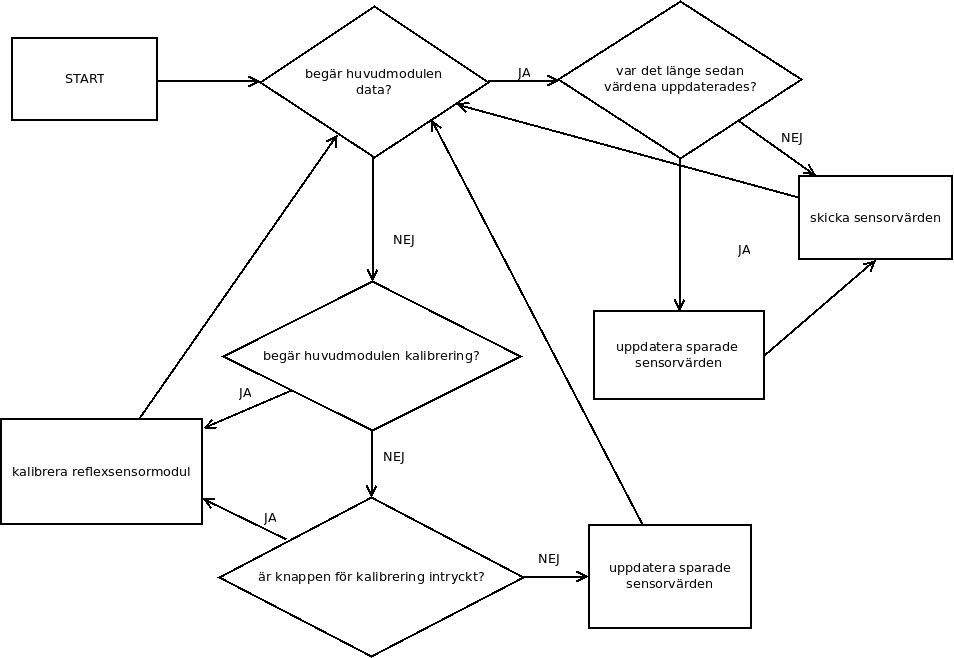
\includegraphics[scale=0.4]{sensorflow}
\caption{Flödesschema för sensormodul.} \label{systemskiss:sensorschema}
\end{figure}

%\end{document}